
\newpage
\section{پیاده سازی کدگذاری ها}
    در این بخش می‌خواهیم نحوه کد کردن اطلاعات
    (مانند یک تصویر) 
    در شبکه های عصبی ضربه‌ای را پیاده سازی و تحلیل کنیم.
    در حوزه علوم اعصاب محاسباتی، روش های کدگذاری برای ترجمه محرک های دنیای واقعی به سیگنال های عصبی که می توانند توسط مدل های محاسباتی پردازش شوند، مهم هستند.
    برای اینکار، روش های مختلفی وجود دارد، مانند روش 
    \lr{time-to-first-spike}، 
    کدگذاری ترتیبی
    \footnote{\lr{Rank-order encoding}}، 
    کدگذاری براساس تاخیر
    \footnote{\lr{Latency encoding}}، 
    کدگذاری براساس همزمانی ضربه ها
    \footnote{\lr{Coding by synchrony}}، 
    کدگذاری اعداد، کدگذاری به روش پواسون
    \footnote{Poisson} 
    و روش های دیگر بسیار که کاربرد های مختلفی دارند.
    (شکل \ref{fig:encoders})
    در این پروژه، ما تمرکزمان را روی سه روش کدگذاری زیر میگذاریم و آن ها پیاده سازی و تحلیل میکنیم:
    \begin{itemize}
        \item روش کدگذاری 
        \lr{time-to-first-spike}
        \item روش کدگذاری مقادیر عددی
        \item روش کدگذاری به کمک توزیع پواسون
    \end{itemize}

    \begin{figure}[!ht]
        \centering
        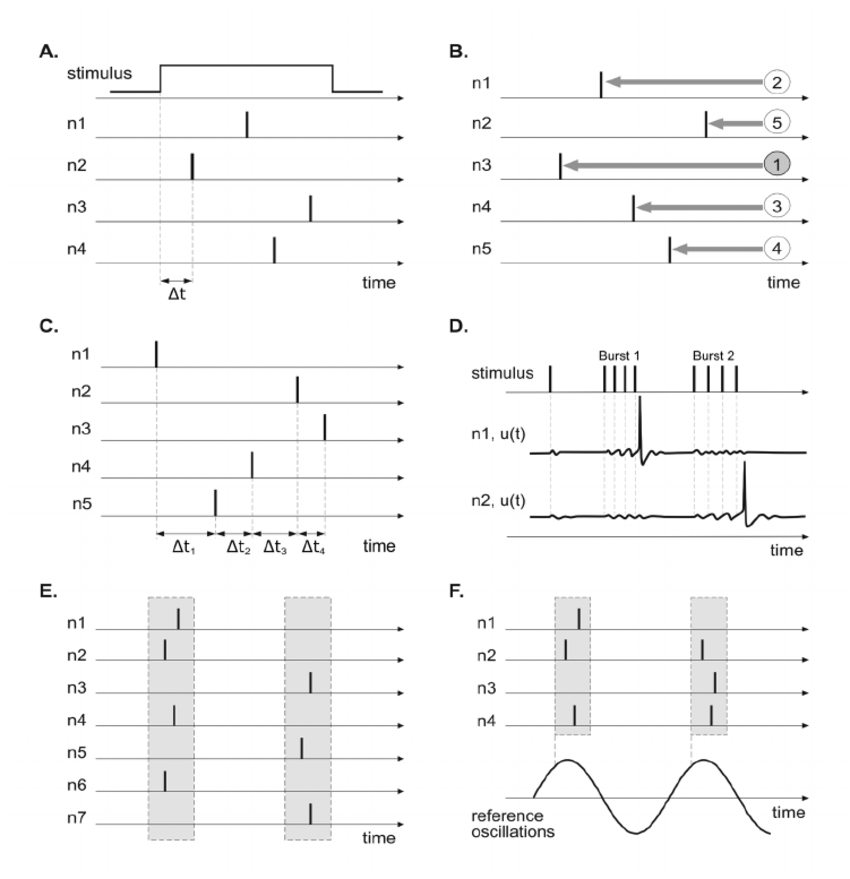
\includegraphics[width=0.4\textwidth]{images/encoders.png} 
        \caption{روش های مختلف کد گذاری. 
        (A) زمان برای اولین ضربه؛ (B) کدگذاری رتبه یا کدگذاری مرتبه ضربه. (C) کدگذاری تأخیر بر اساس زمان دقیق افزایش ها. (D) کدگذاری انفجاری رزونانسی. (E) کدگذاری توسط همزمانی. (F) کدگذاری فازی}
        \label{fig:encoders}
    \end{figure}
    \subsection{کدگذاری به روش 
    \lr{Time-to-first-spike}}
        کدگذاری 
        \lr{Time-to-First-Spike} (TFS)
        روشی است که در آن از زمان اولین اسپایک پس از شروع محرک برای انتقال شدت محرک استفاده می شود. هر چه زمان تا اولین ضربه کوتاه تر باشد، شدت محرک درک شده بیشتر می شود. این روش کدگذاری برای پردازش سریع اطلاعات بسیار مفید است.

        برای کدگذاری 
        Time-to-First-Spike (TFS)
        باید شدت یک محرک را به زمان‌بندی اولین ضربه عصبی تبدیل کنیم. برای اینکار، ابتدا نیاز است با نرمال‌سازی داده‌های ورود حاصل شود که همه مقادیر بین یک آستانه حداقل و حداکثر نگاشت می‌شوند و کمی نیز تنظیم می‌شوند تا از مقادیر شدید جلوگیری شود. فرآیند کدگذاری از یک آستانه استفاده می کند که به مرور توسط یک تابع نمایی کاهشی بر اساس مدت زمان کدگذاری و یک پارامتر
        $\theta$
        کاهش می یابد. این کار به این معنی است که محرک های شدیدتر منجر به ضربه های زودتر می شود. این رمزگذار زمان اولین ضربه را برای هر محرک ثبت می‌کند و مقدار محرک پس از ضربه را برای جلوگیری از کدگذاری مجدد تنظیم می‌کند. نتیجه یک ماتریس باینری است که زمان های افزایش نسبت به شروع محرک را نشان می دهد و به طور موثر اولین پاسخ عصبی قابل توجه را به شدت های مختلف محرک ثبت می کند. به عنوان مثال، یک الگوی ورودی مانند آرایه
        $[100, 70, 30, 10, 0]$
        را با 
        $\theta=1$ 
        کدگذاری کنیم، نمودار 
        $raster$ 
        و نمودار فعالیت به صورت شکل 
        \ref{fig:part1-ttfs-array-encoding}
        خواهد شد.
        \begin{figure}[!ht]
            \centering
            \includegraphics[width=1\textwidth]{plots/part1-ttfs-array-encoding.pdf} 
            \caption{کدگذاری به روش 
            $TTFS$. 
            همانطور که در شکل ملاحظه می شود، با انتخاب کردن 
            $\theta=1$ 
            مقادیر بالای ۱۰۰ در یک لحظه ضربه زده و مقادیر  کمتر در لحظه های بعدی ضربه می زنند. همچنین هر چه مقادیر کمتر می شوند، فاصله بین ضربه ها نیز کمتر می شود.}
            \label{fig:part1-ttfs-array-encoding}
        \end{figure}
        \subsubsection*{تغییر در $\theta$}
        دلیل آنکه مقادیر بالا در یک زمان ضربه زده اند این است که مقدار 
        $\theta$ 
        نسبتا زیاد انتخاب شده است. در شکل 
        \ref{fig:part1-ttfs-array-encoding-change-in-theta}
        ملاحظه میکنیم با انتخاب 
        $\theta=0.01$ 
        فواصل بین ضربه ها با محرک شدیدتر نیز بیشتر می شود. به طور کلی میتوان گفت که کاهش 
        $\theta$ 
        میتواند باعث تفکیک بیشتر بین مقادیر ورودی شود.
        \ref{fig:part1-ttfs-array-encoding-change-in-theta}
        \begin{figure}[!ht]
            \centering
            \includegraphics[width=1\textwidth]{plots/part1-ttfs-array-encoding-change-in-theta.pdf} 
            \caption{کدگذاری به روش 
            $TTFS$. 
            همانطور که در شکل ملاحظه می شود، کاهش پارامتر 
            $\theta$ 
            میتواند باعث بیشتر شدن حساسیت جمعیت به مقادیر مختلف ورودی شود.}
            \label{fig:part1-ttfs-array-encoding-change-in-theta}
        \end{figure}

        \subsubsection*{تغییر در مدت زمان ورودی}
            پارامتر دیگری که در خروجی کدگذاری تاثیر دارد، مدت زمانی ست که ورودی به شبکه داده می شود. این پارامتر تعیین میکند که چقدر طول میکشد تا ورود به نورون ها داده می شود. از این رو، کاهش این پارامتر باعث می شود که الگوی ضربه زدن کدگذاری شده در زمان کمتری به شبکه داده شود و از این رو فواصل بین ضربه ها می تواند کاهش یابد یا حتی در یک زمان ضربه زده شود. از آنجا که در روش کدگذاری 
            $TTFS$ 
            فاصله تا اولین نورونی که ضربه می زند مهم است، انتخاب نادرست این پارامتر میتواند باعث شود تا ورودی به خوبی کدگذاری نشود.
            افزایش این مدت زمان نیز باعث می شود تا فواصل بین ضربه ها بیشتر شود.
            (شکل \ref{fig:part1-ttfs-array-encoding-change-in-duration})

            \begin{figure}[!ht]
                \centering
                \includegraphics[width=1\textwidth]{plots/part1-ttfs-array-encoding-change-in-duration.pdf} 
                \caption{کدگذاری به روش 
                $TTFS$. همانطور که ملاحظه می شود، از راست به چپ، با کاهش مدت زمان ورودی، فاصله بین ضربه ها کمتر شده و زمان ضربه زدن نورون ها فشرده تر می شود. مثلا نورون شماره ۳ و۴ در یک زمان ضربه می زنند.}
                \label{fig:part1-ttfs-array-encoding-change-in-duration}
            \end{figure}
        
        \subsubsection*{کدگذاری تصویر}
            حال یک قدم فراتر گذاشته، و سعی میکنیم یک تصویر را با روش 
            $TTFS$ 
            کدگذاری کنیم. برای انتخاب تصویر، از مخزن دانشگاه واترلو
            \footnote{\href{https://links.uwaterloo.ca/Repository.html}{مخزن تصاویر دانشگاه واترلو}}
            استفاده میکنیم. این تصاویر همگی سیاه و سفید هستند. از این رو میتوانیم کل تصویر را به صورت یک آرایه درنظر بگیریم، به طوری که سطر های تصویر را پشت سر هم ردیف میکنیم. یک تصویر مانند شکل
            \ref{fig:waterloo-sample-image}
            در نظر میگیریم.
            حال یک آرایه به طول 
            $m\times n$ 
            داریم که مقادیر آن بین ۰ و ۲۵۶ هستند. از آنجا که ابعاد تصاویر مخزن، حدود 
            $500\times 500$ 
            هستند، تعداد نورون های مورد نیاز برای کد کردن این ورودی بسیار زیاد خواهد بود و از هدف این پروژه خارج می شود. از این رو ابتدا ابعاد تصاویر را دستکاری کرده و به 
            $10\times 10$ 
            تغییر می دهیم.
            اکنون کافی است مانند بخش قبل ، این آرایه را به عنوان ورودی کدگذاری کرده و به شبکه بدهیم.

            \begin{figure}[htbp]
                \centering
                \begin{subfigure}[b]{0.45\textwidth}
                    \centering
                    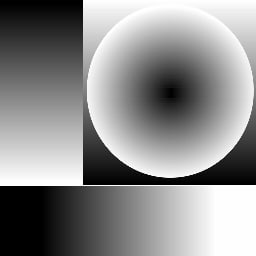
\includegraphics[width=\textwidth]{images/slop.jpg}
                    \caption{تصویر اصلی}
                    \label{fig:waterloo-sample-original}
                \end{subfigure}
                \hfill
                \begin{subfigure}[b]{0.45\textwidth}
                    \centering
                    
\includegraphics[width=\textwidth]{images/slop-resized.jpg}
                    \caption{تصویر کوچک شده}
                    \label{fig:waterloo-sample-resized}
                \end{subfigure}
                \caption{یک تصویر به عنوان محرک}
                \label{fig:waterloo-sample-image}
            \end{figure}
            حال اگر این تصویر را پس از  به عنوان ورودی به شبکه بدهیم نمودار ضربه های کدگذاری شده این تصویر به صورت شکل 
            \ref{fig:part1-ttfs-image-encoding}
            خواهد بود.
            \begin{figure}[!ht]
                \centering
                \includegraphics[width=1\textwidth]{plots/part1-ttfs-image-encoding.pdf} 
                \caption{کدگذاری تصویر به روش 
                $TTFS$. }
                \label{fig:part1-ttfs-image-encoding}
            \end{figure}

            تغییر در مدت زمان ورودی یا 
            $\theta$ 
            نتیجه ای مشابه با تغییراتی که در هنگام کدگذاری آرایه اعداد داشتیم خواهد داشت.

    \subsection{کدگذاری اعداد}
        در این بخش به بررسی یک روش برای کدگذاری اعداد می پردازیم. این روش با استفاده از تابع توزیع نرمال کدگذاری می‌کند. کد گذاری بدین صورت است که برای کد کردن یک عدد، چندین توزیع نرمال مختلف بین یک بازه از اعداد را در نظر گرفته، و مقدار عدد ورودی را به هر یک از این توزیع ها داده و مشاهده میکنیم که این عدد هر یک از این توزیع ها را در کجا قطع می کند. به طور به خصوص فرض کنید می خواهیم یک عدد بین ۱ تا ۱۰، مثلا ۴.۷ را کدگذاری کنیم. حال به ازای هر یک از اعداد صحیح در این بازه یک نورون و یک تابع توزیع نرمال با میانگین آن عدد در نظر میگیریم. حال مقدار هر یک از این توزیع ها در نقطه ۴.۷ را محاسبه میکنیم. هر توزیعی که مقدار بیشتری داشت، بدان معنا است که زودتر ضربه می زند. 
        (شکل 
        \ref{fig:part1-number-encoding}
        را نگاه کنید.)
        \begin{figure}[!ht]
            \centering
            \includegraphics[width=1\textwidth]{plots/part1-number-encoding.pdf} 
            \caption{کدگذاری اعداد. همانطور که در شکل مشاهده می شود، اولین توزیعی که  
            $x=4.7$
            را قطع میکند، توزیع مربوط به نورون ۵ است که در واقعیت نیز عدد ۵ نزدیک ترین عدد صحیح به ۴.۷ 
            است. توزیع های بعدی که  
            $x=4.7$
            را قطع کرده اند به ترتیب مربوط به توزیع با میانگین ۴، توزیع با میانگین ۶، توزیع با میانگین ۳، توزیع با میانگین ۷ و توزیع با میانگین ۳ هستند. بقیه توزیع ها بدلیل داشتن مقدار کم در 
            $x=4.7$ 
            و نزدیک بودن به هم، با توجه به انتخاب  
            $\epsilon$
            با مقدار کم، ضربه ای نزده اند.}
            \label{fig:part1-number-encoding}
        \end{figure}

        زمان ضربه زدن نورون ها به روش های مختلفی می تواند انجام شود. مثلا تابع توزیع  با میانگین ۱، ۲، ۷، ۸، ۹ یا ۱۰ برای عدد ۴.۷ مقدار بسیار کم و نزدیک به همی دارند، و در نتیجه همگی در آخرین لحظات پنجره زمانی
        \footnote{\lr{time window}}
        ضربه خواهند زد. از این رو، باید انتخاب کنیم که آیا نیاز به ضربه زدن همه نورون های بازه داریم یا ضربه زدن مقادیر نزدیک تر کافی است. اینکار توسط انتخاب یک پارامتر مانند 
        $\epsilon$ 
        انجام میگیرد که تعیین میکند مقادیر توزیع ها در 
        $x$  
        از چه مقداری باید بیشتر باشند.
        همچنین برای مقادیر بزرگتر، میتوانیم یک بازه بزرگتر انتخاب کنیم، یا اعداد را به همین بازه ۰ تا ۱۰ مان نگاشت کنیم. همه این روش ها بستگی به استفاده ما دارد. نکته دیگری که در رابطه با این روش کدگذاری وجود دارد، این است که این روش برای کدگذاری داده های زیاد ممکن است مناسب نباشد، چرا که ما به ازای کد کردن هر عدد، نیاز به تعدادی نورون داریم.
        (به عنوان مثال، برای کد کردن تنها ۱۰۰ عدد، نیاز به 
        $100*10=1000$ نورون داریم!)

    \subsection{کدگذاری به کمک توزیع پواسون}
        قبل از اینکه بررسی کنیم کدگذاری به روش پواسون چگونه انجام می شود، بیایید تعریف توزیع پواسون را یکبار با یکدیگر مرور کنیم:
        \textbf{توزیع پواسون: }
        در آمار و احتمال توزیع پواسون یک توزیع احتمالی گسسته است که احتمال اینکه یک حادثه به تعداد مشخصی در فاصلهٔ زمانی یا مکانی ثابتی رخ دهد را شرح می‌دهد؛ به شرط اینکه این حوادث با نرخ میانگین مشخصی و مستقل از زمان آخرین حادثه رخ دهند. 
        (توزیع پواسون همچنین برای تعدادی از حوادث در فاصله‌های مشخص دیگری مثل مسافت، مساحت یا حجم استفاده شود)\cite{Poisson-Distribution-Wikipedia}

        یک متغیر تصادفی گسسته 
        $X$ 
        دارای توزیع پواسون است، با پارامتر 
        $\lambda > 0$
        اگر تابع جرم احتمالی به صورت زیر باشد:
        \begin{equation}
            f(k, \lambda) = P(X=k) = \frac{\lambda^{k}e^{-\lambda}}{k!}
        \end{equation}

        توزیع پواسون را می توان برای سیستم هایی با تعداد زیادی رویداد ممکن که هر کدام نادر هستند اعمال کرد. تعداد چنین رویدادهایی که در یک بازه زمانی ثابت رخ می دهند، در شرایط مناسب، یک عدد تصادفی با توزیع پواسون است.

        معادله را می توان طوری بازنویسی کرد اگر به جای میانگین تعداد رویدادهای 
        $\lambda$
        ، نرخ متوسط 
        $r$ 
        به ما داده شود. که در آن وقایع رخ می دهد. از این رو 
        $r=\lambda t$
        و:
        \begin{equation}
            P(X=k)=\frac{e^{-rt} {(rt)}^{k}}{k!}
        \end{equation}

        ما میدانیم نورون ها ضربه هایی از خود تولید می کنند که این ضربه ها را می توان به عنوان رویدادهای گسسته مدل کرد. به عبارت دیگر زمان هر ضربه را می توان به عنوان یک رویداد تصادفی مشاهده کرد.
        
        با استفاده از توزیع پواسون، می‌توانیم احتمال 
        $P$ 
        مشاهده دقیق 
        $k$ 
        ضربه در بازه زمانی ثابت 
        $t$ 
        را به صورت زیر مدل کنیم:\cite{Poisson-Distribution-Wikipedia}
        \begin{equation}
            P(X=k)=\frac{e^{-\lambda t} {(\lambda t)}^{k}}{k!},
        \end{equation}
        که در آن، 
        \begin{itemize}
            \item $X$ تعداد ضربه ها است.
            \item $e$ عدد اویلر است
            \item $k$ تعداد ضربه هایی است که ما به طور خاص در بازه 
            $t$ 
            به آنها علاقه مندیم.
            \item $\lambda t$ تعداد ضربه های مورد انتظار در بازه 
            $t$ 
            است.
        \end{itemize}

        حال که نحوه عملکرد و پیاده سازی این کدگذاری را فهمیدیم، میتوانیم به سراغ آزمایش کردن کدگذاری ورودی ها برویم. به طور مثال، همانطور مشاهده می شود، به ازای ورودی 
        $[100, 70, 30, 10, 0]$ 
        ضربه های کدگذاری شده به صورت شکل
        \ref{fig:part1-poisson-array-encoding}
        خواهد بود.
        \begin{figure}[!ht]
            \centering
            \includegraphics[width=1\textwidth]{plots/part1-poisson-array-encoding.pdf} 
            \caption{کدگذاری به کمک توزیع پواسون. همانطور که ملاحظه می شود، نورون شماره صفر که بیشترین مقدار، یعنی ۱۰۰ را دارد، بیشترین ضربه را در پنجره زمانی ورودی زده است. نورون های دیگر نیز به نسبت اندازه خود نرخ ضربه داشته اند.}
            \label{fig:part1-poisson-array-encoding}
        \end{figure}

        \subsubsection*{کدگذاری تصویر}
            کدگذاری تصویر به روش پواسون یکی از مواردی است که در ادامه پروژه نیز با آن سر و کار داریم. از این رو می‌خواهیم یک دید کلی نسبت به کدگذاری تصویر به کمک توزیع پواسون داشته باشیم. برای اینکار دوباره از مخزن دانشگاه واترلو استفاده میکنیم و تصویر 
            \ref{fig:waterloo-sample-image}
            استفاده میکنیم. 
            ضربه های کدگذاری شده به صورت شکل
            \ref{fig:part1-poisson-image-encoding}
            خواهد بود.
            \begin{figure}[H]
                \centering
                \includegraphics[width=1\textwidth]{plots/part1-poisson-image-encoding.pdf} 
                \caption{کدگذاری تصویر به کمک توزیع پواسون. شکل بالا مربوط به کدگذاری یک تصویر 
                $10\times 10$ 
                است. تصاویر ابتدا به صورت یک آرایه در می آیند و سپس کدگذاری می شوند. در شکل بالا هر نورون مسئول کد کردن یک پیکسل است.}
                \label{fig:part1-poisson-image-encoding}
            \end{figure}